\graphicspath{{./figures}}

\section{Ground Station}
A block diagram of the system components for the ground station is shown in Figure \ref{fig:gs_system}.

\begin{figure}[!htb]
  \centering
  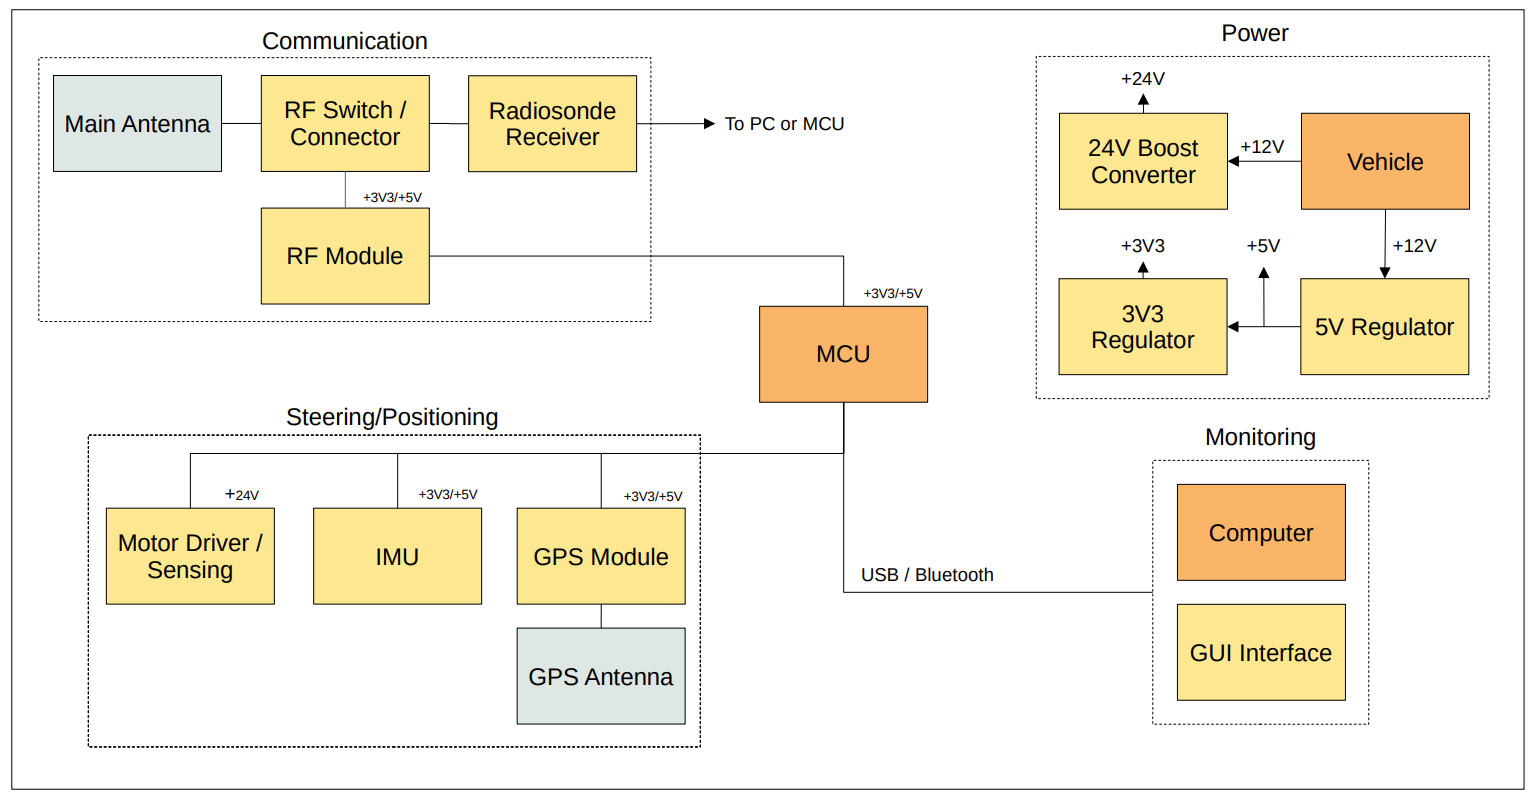
\includegraphics[width=0.8\textwidth]{gs_system}
  \caption{Groud Station System Diagram}
  \label{fig:gs_system}
\end{figure}

\subsection{Power}
The power section consists of two linear regulators, as well as a boost converter. The existing antenna mount has two \textit{NEMA 17 4218S-15} stepper motors, which will be used to steer the ground station in the direction of the satellite. These motors are ideally powered from +24V, and therefore a boost converter will be used to step up the voltage from the car's voltage of +12V. Further, +5V and +3V3 regulators will be provided to power both the MCU and any other ICs, depending on the voltage level they require.

\subsection{Communication}
The communication section consists of the main antenna, as well as the RF control circuitry and connectors. The \textit{RF Switch/Connector} is provided to allow the antenna to be shared between custom and the proprietary communication protocols. Initially, a connector will be used for prototyping. Then, if time allows, a dedicated RF switch will be provided, which will allow for the MCU to control the antenna connection. Both the RF module and the Radiosonde receiver will connect through the RF switch/connector and to the antenna. The Radiosonde will either connect to the PC (if an SDR dongle is used) or to the MCU (if a dedicated receiver is used).

\subsection{Steering and Position}
\begin{figure}[!htb]
    \centering
    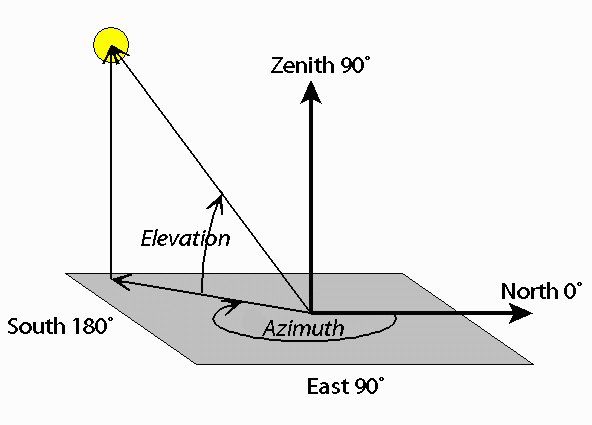
\includegraphics[width=0.4\textwidth]{az_elevation}
    \caption{Azimuthal and Elevation Visualization \cite{site-azElevationVisual}}
    \label{fig:az_elevation}
\end{figure}

Generally, the orientation of the ground station's antenna is described by azimuthal and elevation angles as in Figure \ref{fig:az_elevation}. The resultant two angles should be controllable to a reasonable accuracy such that the antenna can point in a certain direction given

The MCU will drive two motor drivers to orientate the antenna relative to the mount's base. An open-loop prior calibration will be done to convert these motor positions to angles relative 
The ground station requires absolute azimuth angle measurement data, as well as elevation angle/tilt data, in order to orientate itself with respect to its surroundings. The above sensors, as well as a gyroscope, are typically packaged into an \textit{intertial measurement unit} (IMU). 